

%************************************************
\chapter{The Information Bottleneck Principle}\label{ch:ib}

%************************************************

As we already discussed (\cref{sec:communication_problem_setting}), Shannon intentionally left out from information theory\footnote{Which Shannon has always referenced as Communication Theory.} issues of meaning or relevance, and focused on the problem of transmitting information.

Contrarily,~\citeauthor{tishby:1999} argue in~\cite{tishby:1999} that lossy source compression provides a natural quantitative approach to the matter of relevance and, therefore, they use Information Theory itself to address relevance.

This chapter will present the Information Bottleneck Principle, the foundation of the emergent theory subject of this dissertation.

The IB principle approach is related to \acf*{RDT}. Hence, first we will briefly overview RDT as~\citeauthor{tishby:1999} describe it~\cite{tishby:1999,slonim:2002}. Then, we will formally present the IB Principle, its problem setting and solution, and show how it can be seen as a special case of \acl{RDT}.

\section{Rate-Distortion Theory: relevance through a distortion function}\label{sec:RDT}
We know from \cref{eq:shannon_1st_law} that for any rate $R \leq I(X;Y)$ there will be a loss in the reconstructed signal. \acf*{RDT} addresses the problem of determining the rate $R$ that should be communicated over a channel so that the source (input signal $\rvX$) can be approximately reconstructed without exceeding an expected distortion.

\subsection{The \ac{RDT} problem}
\subsubsection{Problem setting}
\begin{enumerate}
	\item Let the discrete random variable $\rvX$ denote the \textbf{source} of vectors randomly drawn from a probability distribution \(p(x)\);
	\item Each vector \(x\sim p(x)\) is a \textbf{message} you want to transmit among a set of possible messages $\aXX,i.e.\  x \in \aXX$ ;
	\item Let another discrete random variable $\rvZ$ denote\footnote{This compressed representation of $\rvX$ is usually denoted by $\rvZ, \rvT$ or $\hat{\rvX}$ } a compressed \textbf{representation} of $\rvX$ ;
	\item This representation is defined by a \textbf{channel}\footnote{A noisy channel and a lossy encoder are equivalents.} $p(z|x)$, a stochastic mapping  between each message $x \in \aXX$ to each code $z \in \aZZ$;
	\item The \textbf{rate} $R$ is the channel capacity, i.e.\ the average number of bits per element $\rx \in \aXX$ needed to specify a compressed element (code) $\rz \in \aZZ$.
	\item Let $d: \aXX \times \aZZ \to \Real^{+}$ be a function that denote the \textbf{distortion measure} between $\rvX$ and its representation $\rvZ$. Examples of distortion measures are the mean square error, $d_{MSE}(x;z)=\langle (x - z)^2 \rangle$ or the Hamming distortion (probability of error) $d_{H}(x,z)=\truth_{[x \neq z]}$.
\end{enumerate}
\subsubsection{Problem Statement}
Given the problem setting above, the \ac*{RDT} problem\footnote{ First defined by Shannon~\citeonly{shannon:1948}.} is to find the minimal number of bits per symbol (rate $R$) that should be communicated over a channel so that the source $\rvX$ can be approximately reconstructed via a representation $\rvZ$ without exceeding an expected distortion $D$, defined by the distortion function $d(x;z)$.

\subsection{Understanding the \ac*{RDT} problem}
The core of the \ac*{RDT} problem is the need for a good compressed representation of a message. From \cref{eq:shannon_1st_law}, any rate $I[\rvZ;\rvX] \leq H[\rvX]$ will imply a loss in the reconstructed signal, an expected distortion,  $\langle d(x;z) \rangle$.

As we have seen in \cref{noisy_channel_theorem}, low values of $I[\rvZ;\rvX]$, calculated based on the joint distribution $p(x,y)=p(x)p(z|x)$, imply compact representations, i.e.\ $|\aZZ|$ is small. In the extreme, all messages are translated to the same code: $|\aZZ|=1$ and $I[\rvZ;\rvX]=0$. Contrarily, high values of $I[\rvZ;\rvX]$ imply low compression.  In the extreme, $\rvZ$ simply copies $\rvX$: $I[\rvZ;\rvX]=H[\rvX]$ and $|\aZZ|=|\aXX|$.

If we can compress the input data to any amount of information from $0$ to $H[\rvX]$, what will define the relevance of information is the aditional constraint of the problem: the distortion measure. Given such function, the partitioning of $\rvX$ defined by $p(z|x)$ has the \emph{expected distortion}:
\begin{align}
	\langle d[x;z] \rangle _{p(x,z)} = \sum_{x,z} p(x) p(z|x) d[x;z]
\end{align}

Consequently, we are assuming that the definition of relevance is part of the problem setting. In other words, \ac{RDT} is agnostic on any arbitrary choice of the distortion function. This choice, nevertheless, determines the relevant features of the signal\footnote{About MLT, the same can be said of a learning algorithm loss function, which determines what is relevant to be learned.} and should be somehow related to the task we want to perform with the input. An arbitrary distortion function is, in fact, an arbitrary feature selection~\cite{tishby:1999}.

As we will se further (\cref{sec:IB_principle}),~\citeauthor{tishby:1999}~\cite{tishby:1999} propose a way to cope with this potential pitfall.

\subsection{\ac*{RDT} as a variational problem}\label{RDT problem}
\begin{definition}
	 The \textbf{rate-distortion function}, denoted by $R(D)$ is defined as:
	 \begin{align}
		R(D) \equiv \underset{p(z|x):~ \langle d(x;z) \rangle \leq D}{\min} I[\rvZ;\rvX]. \label{rate-distortion function}
	\end{align}
\end{definition}

Therefore, $R(D)$ is the minimal achievable rate among all normalized conditional distributions, $p(z|x)$, for which the distortion constraint is satisfied. The \emph{rate-distortion function} is a non-increasing convex function of D in the \emph{distortion-compression plane} (\cref{fig:distortion-compression-plane}\footnote{We will explain what $\beta$ means later.})~\cite{cover:2006}.

\blockfigure{distortion-compression-plane}{1}{The rate-distortion function, $R(D)$, in the distortion-compression plane.}

The region above the curve corresponds to all achievable \emph{distortion-compression} pairs, while below the curve is the non-achievable region. Let $\{D, I_{\rvX}\}$ be a \emph{distortion-compression} pair, if it is in the achievable region there is a representation $\rvZ$ with a compression level $I[\rvZ;\rvX]=\Ix$ and an expected distortion of at most $D$. If it is in the non-achievable region, there is no such representation $\rvZ$. This limit on the achievability of representations is a direct consequence of Shannon's laws (\ref{shannon_laws}).

Instead of solving the minimization problem in \eqref{rate-distortion function} exactly, the problem is usually approximated by the following Lagrangian relaxation functional:
\begin{align}
	\mathcal{F}[p(z|x)] = I[\rvZ;\rvX] + \beta \langle d(x;z) \rangle_{p(x,z)},
\end{align}
under the normalization constraint $\sum_z p(z|x)=1, \forall x \in \aXX$.

\begin{theorem}\label{thrm:RDT solution}
	The solution of the variational problem~\cite{tishby:1999}
	\begin{align}
		\frac{\partial \mathcal{F}}{\partial p(z|x)}=0,
	\end{align}
	for normalized distributions $p(z|x)$ is given by the exponential form
	\begin{align}
		p(z|x) = \frac{p(z)}{Z(x,\beta)}\exp (-\beta ~d(x;z)),\label{exponential-form}
	\end{align}
	where $Z$ is the normalization factor (partition function).  The Lagrange multiplier $\beta$ is positive and
	\begin{align}
		\frac{\partial R}{\partial D} = - \beta.
	\end{align}
\end{theorem}
This is an implicit solution\footnote{Implicit solution means a solution in which dependent variable is not separated.} as $p(z)$ on the right-hand side of \cref{exponential-form} depends on $p(z|x)$\footnote{$p(z)=\sum_{x,z} p(z|x)~p(z)$}.

\section{The IB Principle: relevance through a target variable}\label{sec:IB_principle}
The problem of extracting a relevant summary of data depends on a suitable definition of relevance. The main weakness of the \ac{RDT} approach is that it addresses relevance through a distortion function that is not related to a specific task at hand.

The \textbf{IB Principle}, suggested by \citeauthor{tishby:1999}\cite{tishby:1999} introduces an alternative approach: defining a ``target'' variable is simpler and more direct than defining a distortion measure.

For example, in speech compression\footnote{By the time of~\citeonly{tishby:1999} publication, Tishby was working on speech-related problems.}, any compression beyond the signal's entropy cannot be perfectly reconstructed; it is a lossy compression. On the other hand, a transcript has orders of magnitude lower entropy than the acoustic waveform, which means that for the task of understanding what has been transmitted, it is possible to compress the signal \emph{much} further without losing any information about meaning~\cite{tishby:1999}.

\begin{figure}
	[htb] \centering
	\includegraphics[width=
	\textwidth]{ib_setting}
	\caption{The IB problem setting.}\label{fig:ib_problem_setting}
\end{figure}

In many situations, we have access to an additional variable that determines what is relevant. If we want to recognize cats in pictures, maybe we do not need a 360~kb picture as depicted on the left in \cref{fig:ib_problem_setting}; the 5~kb representation on the right may suffice. The exact representation would not be sufficient for the task of recognizing the breed of the cat, in any case. Relevance is task-dependent.


\subsection{The IB Problem Setting}\label{ib_problem_setting}
\subsubsection{Definitions}
\begin{enumerate}
	\item Let $\rvX$ be a random variable that denotes the \textbf{Source} \footnote{The IB problem is a one-shot coding problem, the operations are performed letterwise~\citeonly{zaidi:2020}.} of \textbf{messages} $\rx \in \sA_{\rvX}$;
	\item Let $\rvY$ be a random \textbf{relevant variable}  (or \textbf{Target}) which defines the intended meaning $p(y|x)$ of the message $x$;
	\item Let $\rvZ$ be an \textbf{information bottleneck} variable, the representation, that obeys the Markov chain $\rvY \leftrightarrow \rvX \leftrightarrow \rvZ$;
	\item Let the conditional p.d.f $p(z|x)$ be the \textbf{encoder}, \ie a stochastic mapping from each value of $x \in \sA_{\rvX}$ to a codeword $z \in \sA_{\rvZ}$;
	\item $I(\rvX ; \rvZ)$ is the \textbf{rate} (or compression level) of the encoder, and reflects how much the bottleneck representation  $\rvZ$ compresses $\rvX$;
	\item Let the conditional p.d.f $p(y|z)$ be the \textbf{decoder}, \ie a stochastic mapping from each value of $z \in \sA_{\rvZ}$ to a prediction $\hat{y} \in \hat{\rvY}$;
	\item $I(\rvZ ; \rvY)$ is the \textbf{relevant information} that the compressed representation $\rvZ$ keeps from the label variable $\rvY$;
\end{enumerate}

  \subsubsection{Assumptions}\label{assumptions}
  \begin{enumerate}
    [i.]
    \item The random variables $\rvX$, $\rvY$ and $\rvZ$ are discrete;
    \item $\sA_{\rvX}$, $\sA_{\rvY}$ and $\sA_{\rvZ}$ are finite sets;
    \item $\rvX$ and $\rvY$ are dependent and the joint distribution $p(\rvX=x, \rvY=y)$ is known;
		\item The source $\rvX$ is an ergodic process\footnote{The \emph{ergodic} property means statistical homogeneity~\cite{shannon:1949}:~ its statistical properties can be deduced from a single, sufficiently long, random sample of the process.}, therefore $x \sim p(x)$ are not necessarily mutually independent.
		\item The encoder and the decoder are stochastic mappings \footnote{Notice that given the Markov chain $\rvY \leftrightarrow \rvX \leftrightarrow \rvZ$, due to reparemetrization invariance (Theorem \ref{th:reparemetrisation_invariance}), a deterministic mapping of the data does not throw out information, i.e. \ let $f:\aXX \to \aYY$ be deterministic, $I[f(\rvX);\rvY]=\IXY$.}.
  \end{enumerate}
\subsubsection{Problem statement}
% The \emph{information bottleneck} consists of finding a representation $\rvZ$ for $\rvX$ that preserves the maximum information about $\rvY$, squeezing the information that $\rvX$ contains on $\rvY$ through a \emph{bottleneck} $\rvZ$ defined by a limited set of codewords $\sA_{\rvZ}$.
The \emph{information bottleneck problem} consists of finding an encoder $p(z|x)$ that produces a codebook  $\rvZ$ that compress $\rvX$ as much as possible, i.e.\ $I(\rvX ; \rvZ)$ is minimal, while keeping the \emph{relevant information} of $\rvX$ for the task of predicting $\rvY$, $I(\rvZ;\rvY)$. In other words, the representation $\rvZ$ acts like a \textbf{bottleneck} that "squeezes" the relevant information that $\rvX$ contains about the target $\rvY$ in a compressed form, hence the name "information bottleneck".
\subsection{Relation to other Information Theory Problems}
Connections between problems allow extending ideas from one setup to another. In this regard, the IB problem is closely related to other coding problems like the \emph{Indirect} or \emph{Remote Source-coding problem}, also known as the \emph{CEO Problem}, and the \emph{privacy funnel problem}\cite{zaidi:2020}.
\subsection{Relation to Minimum Sufficient Statistics}
As we have said before,  a \textbf{statistic} is a function of a random variable that does not depend on its parameters. In the IB problem, the target variable is what we want to predict. $\rvY$ acts as a parameter of $\rvX$ and  $\rvZ \ind \rvY$. Thus, \emph{the representation $\rvZ$ is a statistic of $\rvX$}.

For $\rvZ$ to be a \textbf{sufficient statistic} of $\rvX$ w.r.t. $\rvY$, it must preserve all relevant information in $\rvX$, $I[Y;X]=I[Z;X]$. In other words, no other statistic of $\rvX$ can provide any additional information as to the value of $\rvY$ than $\rvZ$ does.

The representation is \textbf{minimal} if it is the smallest among all possible representations.

Therefore, we can say that the information bottleneck is the problem of finding the \emph{minimum sufficient statistics} of the random variable $\rvX$ w.r.t $\rvY$, and therefore, IB Lagrangian gives the minimum approximately sufficient statistic.
\section{The IB functional}\label{sec:ib_functional}
As in {RDT}, the compactness of the representation is measured by $I[\rvZ;\rvX]$.  The distortion upper-bound constraint, however, is replaced by a lower bound constraint over the \emph{relevant information}, $I[\rvZ;\rvY]$\cite{slonim:2002}.

\begin{definition} The \textbf{IB functional}, also know as the \emph{IB Curve} or \emph{relevance-compression function}, is the functional that express the IB problem\cite{bachrach:2003}:
\begin{align}
	R^{(\text{IB})}(I_{\rvY}) &= \underset{p(z|x):~ I[\rvZ;\rvY]\geq I_{\rvY}}{\min} I[\rvZ;\rvX],\\
	\text{or alternatively:} \nonumber                                              \\
	I_{\rvY}^{(\text{IB})}(R)&= \underset{p(z|x):~ I[\rvZ;\rvX]\leq R}{\max} I[\rvZ;\rvY],
\end{align}
where the random variables form a Markov chain $\rvY \leftrightarrow  \rvX \leftrightarrow  \rvZ$ and the minimization is over all the normalized conditional distributions $p(z|x)|\sum_x p(z|x)=1$ for which the constraint is satisfied.
\end{definition}
A straighforward observation is that the Markovian relation characterizes $p(z)$ and $p(y|z)$ through\cite{slonim:2002}
\begin{align}
	\begin{cases}
		p(z) = \sum_{x,y} p(x,y,z) = \sum_x p(x)p(z|x)  \\
		p(y|z) = \frac{1}{p(z)}\sum_x p(x,y,z) = \frac{1}{p(z)}\sum_x p(x,y) p(z|x).\label{observation}
	\end{cases}
\end{align}

Moreover, the plane where the horizontal axis corresponds to $I[\rvZ;\rvX]$ and the vertical axis to $I[\rvZ;\rvY]$, named \textbf{information plane} (see Figure \cref{fig:information-plane}), is the natural equivalent to the distortion-compression plane in \acl{RDT} (see \cref{fig:distortion-compression-plane})\footnote{The horizontal and vertical axis are inverted for consistency with how~\cite{tishby:2015} define the information plane. Therefore, whereas the rate-distortion function is convex, the IB curve is concave.}. Let the pair ${R, \Iy}$ denote some levels of compression and relevant information, respectively. If this pair is located below the curve, there is some compressed representation $\rvZ$ with a compression level $R=I[\rvZ;\rvX]$ and relevant information $\Iy=I[\rvZ;\rvY]$. The points laying on the IB Curve are the optimal representations for a certain level of relevant-information (or precision) $\Iy$ or a certain level of compression (or complexity) $R$.


\begin{figure}
	[htb] \centering
	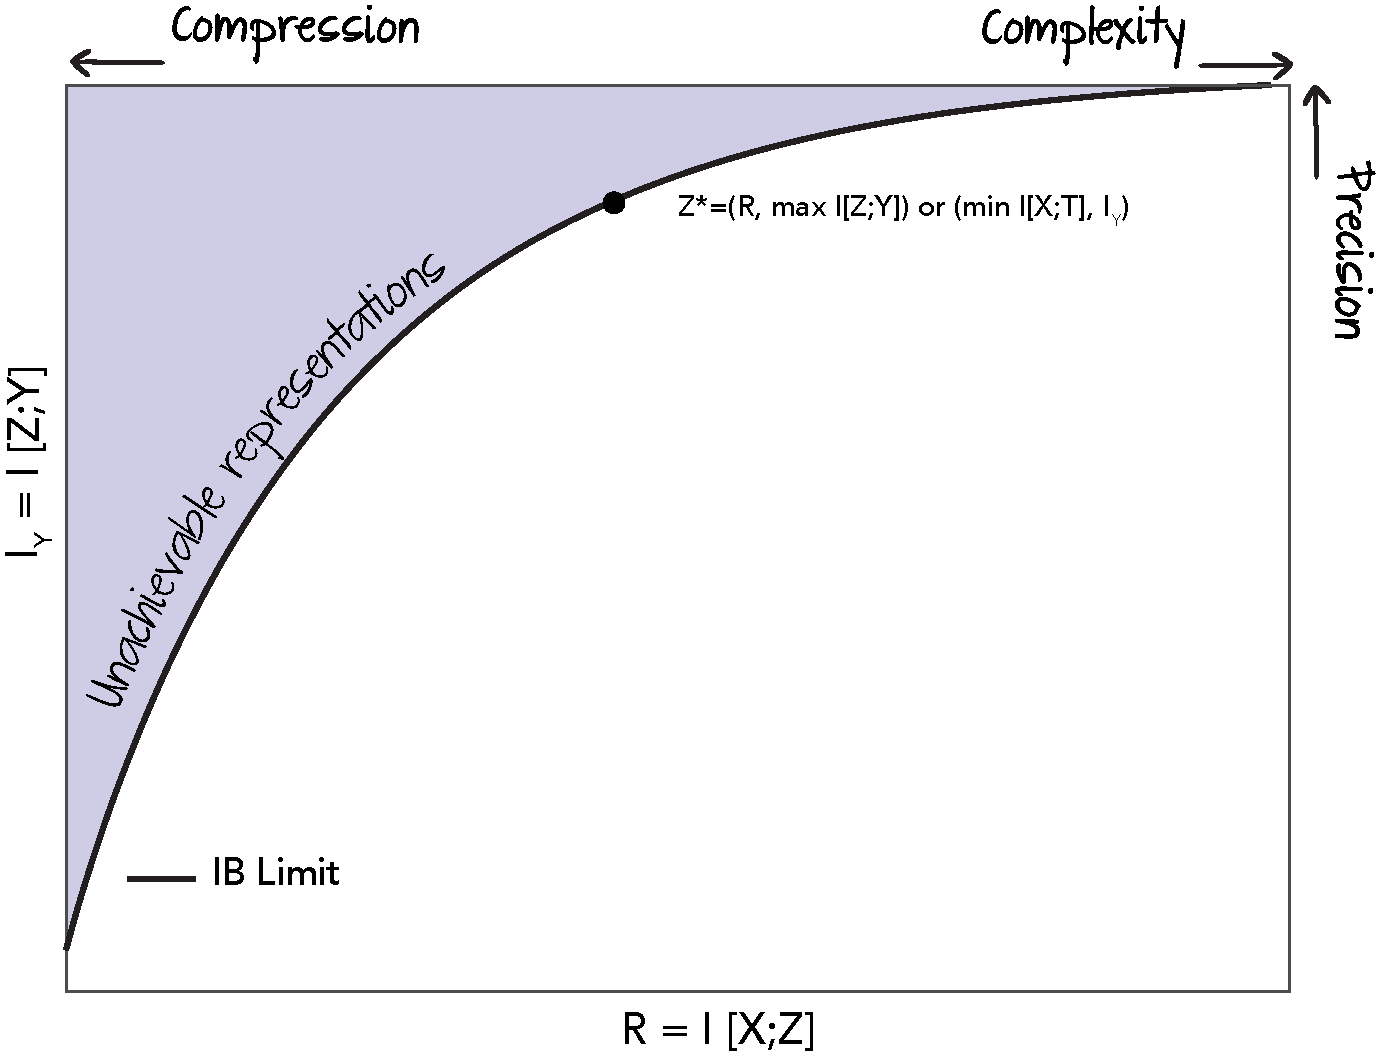
\includegraphics[width=
	.7\textwidth]{information-plane}
	\caption{The IB Curve, $R^{\text{(IB)}}(D)$, in the information plane.}\label{fig:information-plane}
\end{figure}
\section{The IB Problem Relaxation}\label{sec:ib_problem_relaxation}
The Lagrangian relaxation of the IB functional is also a variational problem:

\begin{align}
	\LH_{\beta}^{\text{(IB)}}[p(z|x)] = \IZX - \beta \IZY, \label{IB_Lagrangian}
\end{align}
where $\beta$ is the Lagrangian multiplier attached to the constrained relevant information\cite{tishby:1999}.

At $\beta=0$, no feature of the signal is relevant, and all messages are quantized (compressed) to a single point. At $\beta=\infty$, the solution is pushed toward arbitrarily detailed quantization (no compression). "By varying the (only) parameter, $ \beta$, one can explore the tradeoff between the preserved meaningful information and compression at various resolutions"\cite{tishby:1999}.
% Relevant information
% For each value $x \in X$ we seek a stochastic mapping to a codeword $z$ in a codebook $Z$, characterized by the p.d.f. $p(z|x)$, which induces a soft partitioning of $X$ in which each block is associated with one element $z \in Z$, with probability \[p(z)=\sum_x p(x) p(z|x).\]

% The average volume of elements of $X$ mapped to the same codeword is $2ˆ{H(X|Z)}$, where
% \[ H(X|Z)= - \sum_{x \in X}p(x) \sum_{z \in Z} p(z|x) \log p(z|x) \] is the conditional entropy of $X$ given $Z$.

Unlike the case of the \cref{RDT problem}, in the IB problem, the constraint on the meaningful information is \emph{nonlinear} in the mapping  $p(z|x)$, and it is a much harder variational problem. Notably, there is an analytical solution for \Eqref{IB_Lagrangian}. For the sake of clarity, before deriving this exact solution, we will show how IB can be seen as a particular case of \ac*{RDT}. This development will further help us to derive the analytical solution easily.

\section{IB problem as a special case of the RDT problem}
From the \acf{DPI}, \(I[\rvX;\rvY] \geq I[\rvZ;\rvY]\). Therefore, we can consider that the relevant information of $\rvX$ not captured by the representation $\rvZ$ is a natural choice for the expected distortion, as it represents a distortion in bits.
\begin{align}
	\langle d[x;z] \rangle = I[\rvX;\rvY]-I[\rvZ;\rvY]\geq 0
\end{align}
From this definition, we can derive the following theorem:
\begin{theorem}
If $\langle d[x;z] \rangle_{p(x,z)}=I[\rvX;\rvY]-I[\rvZ;\rvY]$, then $\\d[x;z] = \KL(p(y|x)~||~p(y|z))$.
\end{theorem}
\begin{proof}
	\begin{align}
		&\langle d[x;z] \rangle_{p(x,z)} =I[\rvX;\rvY]-I[\rvZ;\rvY]\nonumber\\
		&=\sum_{x,y} p(x, y) \log \frac{p(x,y)}{p(x) p(y)} - \sum_{z,y} p(z, y) \log \frac{p(z,y)}{p(z) p(y)}.
	\end{align}
	Since $p(a,b) = p(b|a) p(a)$, we have:
	\begin{align}
		=&\sum_{x,y} p(y|x) p(x) \log \frac{p(y|x)\cancel{p(x)}}{ \cancel{p(x)}p(y)} -\sum_{z,y} p(y|z) p(z) \log \frac{p(y|z)\cancel{p(z)}}{ \cancel{p(z)}p(y)}.
	\end{align}
	From \eqref{observation} :
	\begin{align}
		=&\sum_{x,y} p(y|x) p(x) \log \frac{p(y|x)}{ p(y)} - \sum_{z,y,x} \frac{p(y|x) p(z|x) p(x) \cancel{p(z)}}{\cancel{p(z)}}~\log \frac{p(y|z)}{ p(y)}\\
		=&\sum_{x,y} p(y|x) p(x) \log \frac{p(y|x)}{ p(y)} - \sum_{z,y,x} p(y|x) p(z,x)~\log \frac{p(y|z)}{ p(y)}.
	\end{align}
	From the normalization constraint, $\sum_{z} p(z|x)=1$:
	\begin{align}
		=&\cancelto{\sum_{z} p(z|x)}{1} \cdot \sum_{x,y} p(x) p(y|x) \log \frac{p(y|x)}{ p(y)} - \sum_{z,y,x} p(y|x) p(z,x)\log \frac{p(y|z)}{ p(y)}\\
		=&\sum_{z,x} p(z|x)p(x) \left[\sum_{y}  p(y|x) \log \frac{p(y|x)}{ p(y)}\right] - \sum_{z,x} p(x,z) \left[ \sum_{y} p(y|x) \log \frac{p(y|z)}{ p(y)}\right]\\
		=&\sum_{z,x} p(x,z) \left[\sum_{y}  p(y|x) \left(\log \frac{p(y|x)}{ p(y)}- \log \frac{p(y|z)}{ p(y)}\right)\right]\\
		=&\sum_{z,x} p(x,z) \left[\sum_{y}  p(y|x) \left(\log \frac{p(y|x) \cancel{p(y)}}{ \cancel{p(y)} p(y|z)}\right)\right]\\
		=&\E_{p(z,x)}  \KL{\left(~p(y|x)~ ||~ p(y|z)~ \right)}.
	\end{align}
	Therefore
	\begin{align}
		\langle d[x;z] \rangle_{p(x,z)} &= \langle \KL{\left(~p(y|x)~ ||~ p(y|z)~ \right)} \rangle_{p(x,z)}\\
		d[x;z] &= \KL{\left(~p(y|x)~ ||~ p(y|z)~ \right)}
	\end{align}
\end{proof}

\section{Information Bottleneck Solution}% Analytical solution

Theorem \ref{thrm:RDT solution} characterizes the general form of the optimal solution to the rate-distortion problem. As we showed that the IB problem could be seen as a special case of the RDT problem, the IB solution is straightforward:\footnote{The analytical solution to the IB problem is sometimes called the self-consistent equations.}
\begin{theorem}\label{thrm:IB solution}
	The analytical solution of the variational problem
	\begin{align}
		\frac{\partial \mathcal{L}_{\beta}^{\text{(IB)}}[p(z|x)]}{\partial p(z|x)} = 0,
	\end{align}
	for normalized distributions $p(z|x)$ is given by the exponential form
	\begin{align}
		\begin{cases}
		p(z|x) &= \frac{p(z)}{Z(x,\beta)}\exp (-\beta ~\KL{\left(~p(y|x)~ ||~ p(y|z)~ \right)}),\\
		p(z) &= \sum_{x,y} p(x,y,z) = \sum_x p(x)p(z|x)  \\
		p(y|z) &= \frac{1}{p(z)}\sum_x p(x,y,z) = \frac{1}{p(z)}\sum_x p(x,y) p(z|x).
		\end{cases}
	\end{align}
	where $Z$ is the normalization factor (partition function).  The Lagrange multiplier $\beta$ is positive and
	\begin{align}
		\beta = \frac{\partial I[Z;Y]}{\partial I{Z;X}}.
	\end{align}
\end{theorem}
\begin{proof}
	Apply $d[x;z] = \KL{\left(~p(y|x)~ ||~ p(y|z)~ \right)}$ to theorem \ref{thrm:RDT solution}.
\end{proof}